\subsection{Pseudocódigo}

Modelamos el problema utilizando grafos en donde los nodos representan a los clientes y a las fábricas y las aristas con peso a las rutas. Internamente, tenemos listas de adyacencia, es decir, cada nodo tiene una lista de sus nodos adyacentes.

Para resolver este ejercicio utilizamos el algoritmo de Prim con algunas modificaciones. Dado un grafo G=(V,E), el algoritmo de Prim encuentra un subconjunto T de E tal que utilizando solamente las aristas de T, todos los nodos deben quedar conectados, y además la suma de las aristas de T debe ser tan pequeña como sea posible. Sea G' un nuevo grafo con los nodos de G y las aristas de T, definimos a G' como $arbol$ $generador$ $minimo$. La idea de la utilización de este algoritmo nace de la necesidad de obtener un bosque de árboles generadores mínimos. En la solución no deben quedar necesariamente todos los nodos (fábricas o clientes) conectados. Esto ocurre en la solución presentada en la figura 2. Aquí no disponemos de un árbol sino que tenemos dos bosques de AGM por separado.

A continuación un pseudocódigo del algoritmo de Prim del cual iremos mostrando las modificaciones hechas.

\begin{algorithm}[H]
\caption{Prim}\label{ej1}
\begin{algorithmic}[1]
\Procedure{Prim}{$G=(V,E)$}
	\State T  $\shortleftarrow$ $\emptyset$
	\State B $\shortleftarrow$ $\{$un nodo arbitrario de V$\}$
	\While{$B \neq V$}
		\State buscar $e=\{u,v\}$ de longitud mínima tal que u $\in$ B y v $\in$ V-B
		\State T $\cup$ $\{e\}$
		\State B $\cup$ $\{v\}$
	\EndWhile
	\State return T
\EndProcedure
\end{algorithmic}
\end{algorithm}

%En este ejercicio ignoramos las aristas que comunican dos fábricas entre si ya que no pertenecerán a la solución hallada. Esto se debe a que solamente nos interesa conectar clientes con fábricas de forma óptima

Teniendo en cuenta que la configuración inicial del problema no nos garantiza que todos los nodos tengan al menos un nodo conectado (pueden haber fábricas aisladas) y considerando que la solución final hallada no debe ser necesariamente un árbol, el algoritmo tendrá que  inicializar el conjunto B con todas las fábricas disponibles e ir eligiendo aristas de longitud mínima que no comuniquen fábricas con fábricas. Entonces, el pesudocódigo quedaría de la siguiente forma:

\begin{algorithm}[H]
\caption{PrimModificado}\label{ej1}
\begin{algorithmic}[1]
\Procedure{PrimModificado}{$G=(V,E), int \ cantClientes,int \ cantFabricas$}
	\State T  $\shortleftarrow$ $\emptyset$
	\State B $\cup$ $\{$todos los nodos que representan a una fábrica$\}$
	\While{$\#T \neq cantCientes$}
		\State buscar $e=\{u,v\}$ de longitud mínima tal que u $\in$ B y v $\in$ V-B de manera que $e$ no una dos fábricas.
		\State T $\cup$ $\{e\}$
		\State B $\cup$ $\{v\}$
	\EndWhile
	\State return T
\EndProcedure
\end{algorithmic}
\end{algorithm}

Observemos cómo se comportaría el algoritmo presentando para el ejemplo de la figura 1:

\begin{figure}[H]
 \centering
  \subfloat[Como los nodos 1 y 2 son fábricas, las aristas de posible elección serán todos los clientes que estén conectados a ellas.]{
   \label{}
    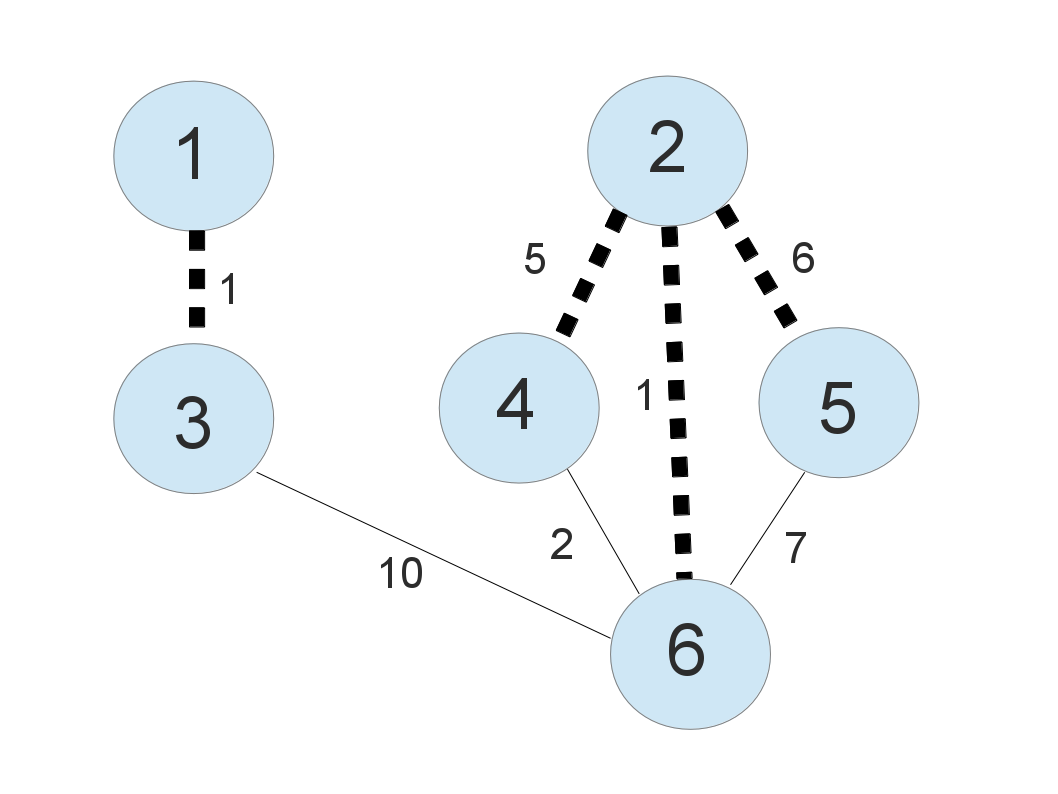
\includegraphics[scale=0.2]{ej3/imgs/graph1_1era.png}}
  \subfloat[Habiendo elegido la arista (1,3), se agrega una arista más a las posibles: (3,6).]{
   \label{}
    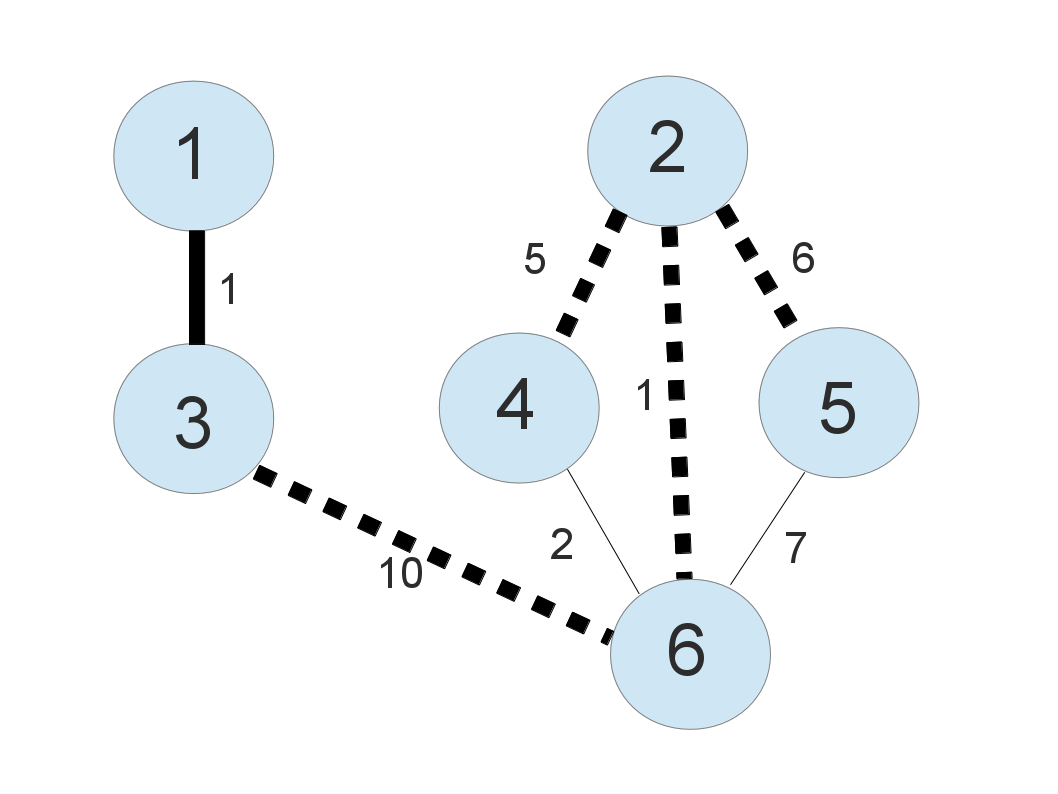
\includegraphics[scale=0.2]{ej3/imgs/graph1_2da.png}}
  \subfloat[Eligiendo (2,6) se despliegan nuevas aristas para elegir y la (3,6) ya no puede ser elegida porque los nodos de ambos extremos ya se encuentran en el conjunto B.]{
   \label{}
    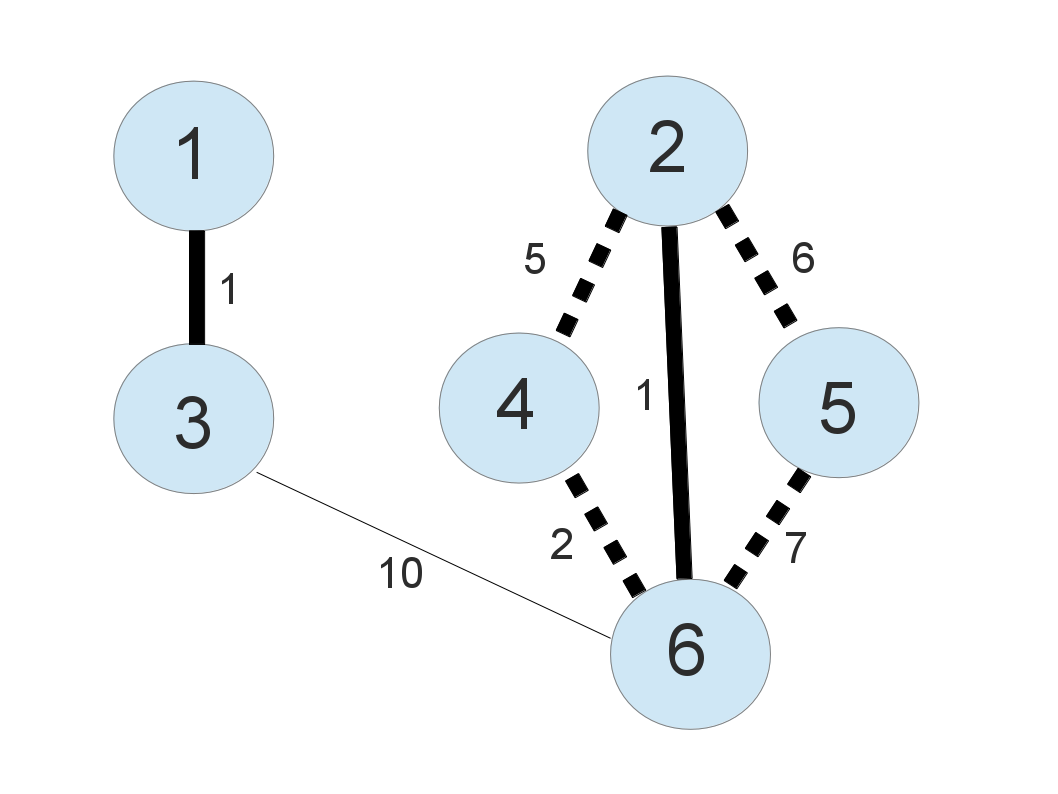
\includegraphics[scale=0.2]{ej3/imgs/graph1_3era.png}}
  \subfloat[Elegimos la (4,6) y la (2,5) ya no puede ser elegida.]{
   \label{}
    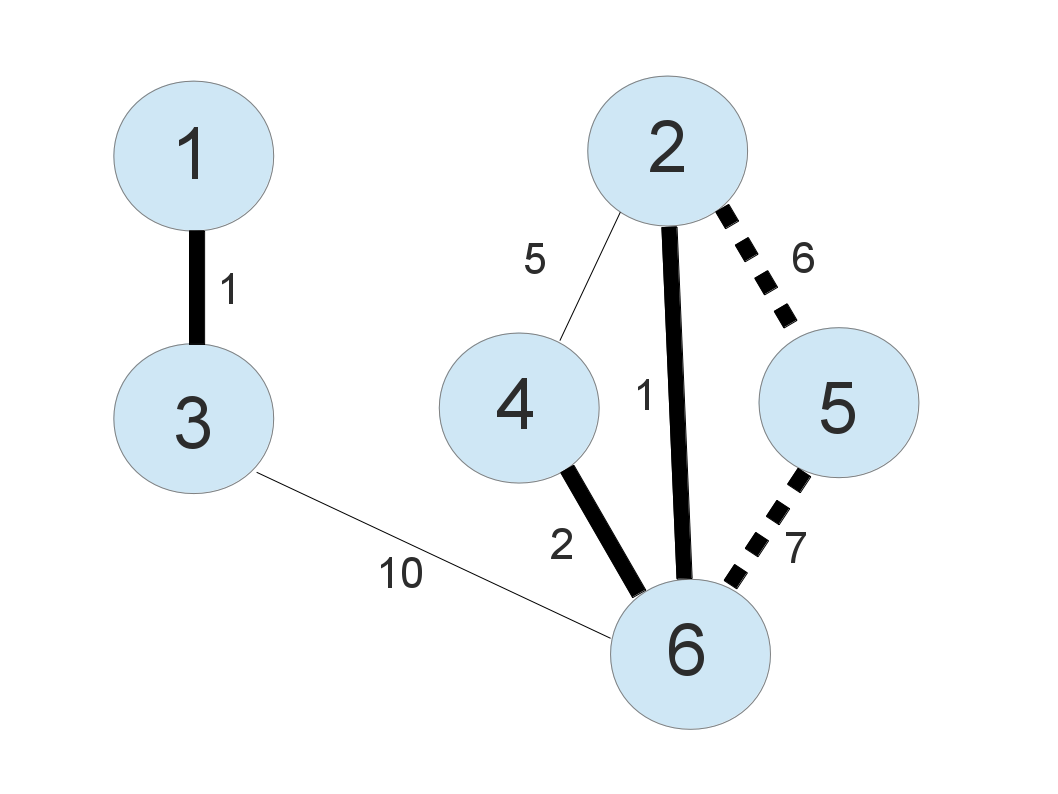
\includegraphics[scale=0.2]{ej3/imgs/graph1_4ta.png}}
  \subfloat[Por último, tomamos la arista (2,5) y llegamos a la solución.]{
   \label{}
    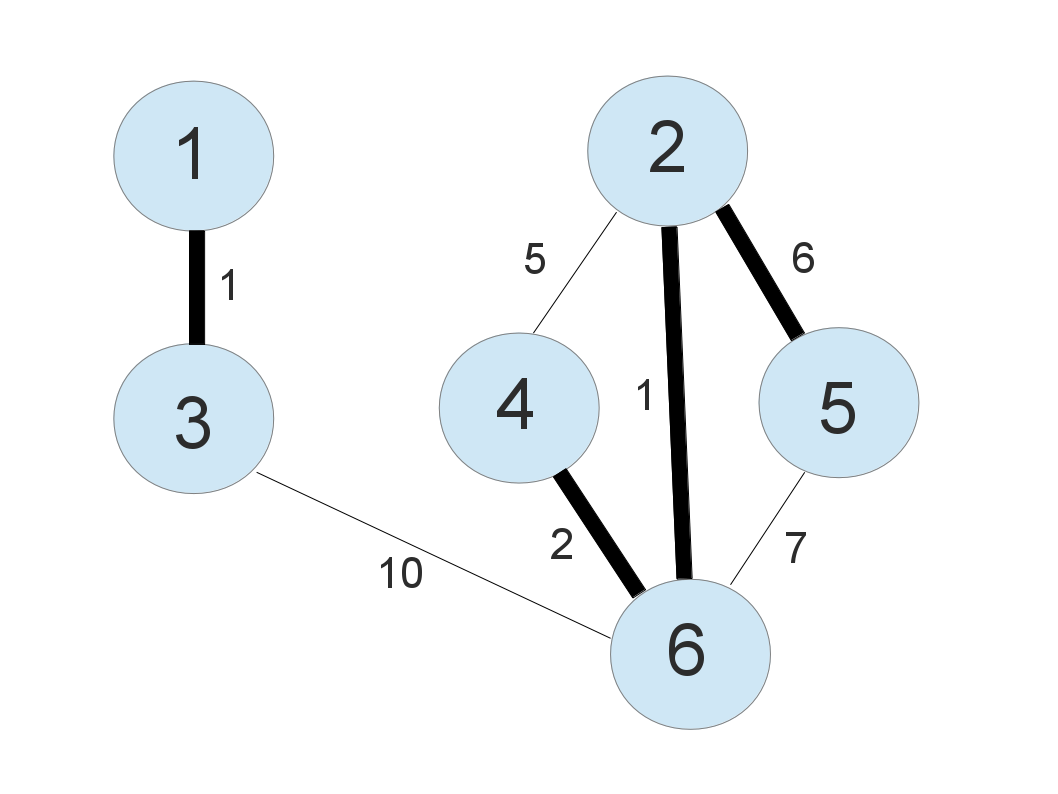
\includegraphics[scale=0.2]{ej3/imgs/graph1_sol.png}}
 \caption{Iteraciones del algoritmo. Las aristas punteadas son aquellas que pueden ser elegidas en la iesima iteración del algoritmo. Las marcadas en negro son las elegidas.}
 \label{}
\end{figure}

Los bosques obtenidos en la solución del algoritmo de Prim modificado van creciendo a partir de varias raíces (fábricas). En cada fase se añade una nueva rama a alguno de los bosques y se detiene cuando se tienen tantas aristas como clientes. Esto último puede demostrarse por inducción. Si disponemos de una fábrica y un cliente, la cantidad de aristas totales de la solución será 1 conectando el cliente con la fábrica de forma directa. Suponiendo que vale para n clientes y j fábricas veamos que vale para n+1 clientes. Si conectamos el nuevo cliente a una fábrica tendremos n+1 aristas en la solución. Si por el contrario lo unimos a un cliente i, nos garantizamos de que se encuentra provisto por alguna fábrica ya que el cliente i también lo está. Aquí también estaríamos agregando una arista por lo cual llegaríamos también a n+1.


